% Allow relative paths in included subfiles that are compiled separately
% See https://tex.stackexchange.com/questions/153312/
\providecommand{\main}{..}
\documentclass[\main/thesis.tex]{subfiles}

\begin{document}

% \chapter{Multilabel 12-Lead Electrocardiogram Classification Using Beat to Sequence Autoencoders}
\chapter{Beat to Sequence Autoencoders}
\chaptermark{DLAutoEncoder}
\label{chp:dl_autoenc}

In this chapter, I propose an approach for the 12-lead \gls{ecg} classification problem using a series of autoencoders to learn a dense embedding representation underlying record.
The work contained in this chapter is adapated from ``Multilabel 12-Lead Electrocardiogram Classification Using Beat to Sequence Autoencoders'' and has been submitted to the IEEE International Conference on Acoustics, Speech, and Signal Processing (ICASSP) 2021.
This work has manuscript revisions from Dr.\ Abram Hindle and Dr.\ Sunil Vasu Kalmady, as well as the contribution of Figure~\ref{fig:aenc_methodology} from Amir Salimi.

% Takeaways
\paragraph{What to take away from this chapter}
\begin{itemize}
    \item our beat to sequence autoencoder approach is statistically more sensitive than the XGBoost ensemble method in detecting \gls{irbbb}, \gls{lanfb}, \gls{pr}, and \gls{rad}.
    \item however, for overall \gls{ecg} classification metrics, the beat to sequence autoencoder is a less effective classifier than the prior XGBoost ensemble approach
    \item future work, combining the benefits of the autoencoder embeddings and the shallow tree classifier may lead to a better overall classifier 
\end{itemize}

% ==================================
% Begin ICASSP-2021 Paper Submission
% ==================================

\begin{abstract}
The 12-lead electrocardiogram (ECG) measures the electrical activity of the heart for physicians to use in diagnosing cardiac disorders.
This paper investigates the multi-label, multi-class classification of ECG records into one or more of 27 possible medical diagnoses.
Our multi-step approach uses conventional physiological algorithms for segmentation of heartbeats from the baseline signals.
We stack a heartbeat autoencoder over heartbeat windows to make embeddings, then we encode this sequence of embeddings to make an ECG embedding which we then classify on.
We utilize the public dataset of 43,101 available ECG records provided by the \emph{PhysioNet/CinC 2020 challenge}, performing repeated random subsampling and splitting the available records into 80\% training, 10\% validation, and 10\% test splits, 20 times.
We attain a mean test split challenge score of 0.248 with an overall macro $\text{F}_1$ score of 0.260 across the 27 labels.
\end{abstract}
%
% \begin{keywords}
% electrocardiogram, signal autoencoder, signal embedding, multi-label classification, PhysioNet/CinC
% \end{keywords}
%
\section{Introduction}

\begin{figure}[t]
    \centering
    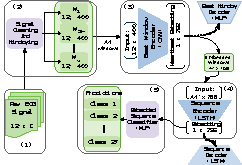
\includegraphics[width=12cm]{figure/aenc_methodology.pdf}
    \caption{Methodology overview. From (1) $\mathcal{L}$-sized ECG signal, we (2) extract $\mathcal{M}$ heartbeat windows prior to (3) heartbeat \& (4) sequence autoencoding. Finally we (5) pass our sequence embedding to the classifier to output our 27 predictions.}
    \label{fig:aenc_methodology}
\end{figure}

Although the electrocardiogram (ECG) is an effective tool for detecting cardiac diseases, the analysis of the ECG is a specialized skill requiring training and human over-reading of computerized interpretations.
Our work extends the \emph{PhysioNet/CinC 2020 Challenge}~\cite{physionet_challenge_2020} involving multi-label classification of ECGs, which are 12 channel 500-1000Hz signals with 27 labels indicating cardiologist diagnoses.
Our novel component is the use of sequentially windowed embeddings to classify the ECGs.
We train a two component signal autoencoder algorithm, encoding the heartbeat windows, then the sequence of window embeddings, before using the sequence bottleneck embedding for classification.
We extend and compare against our prior work by learning autoencoded features rather than using manually engineered features~\cite{wong2020CINC-multilabel-ECG}.

\section{Related Work}

We are inspired by prior work that uses autoencoders to generate features for signal classification~\cite{8688435,7752836}.
Recent advancements in machine learning and available data have heralded an influx of multi-lead ECG classification algorithms~\cite{ribeiro2020,CHEN2020100886,9206538,BALOGLU201923,8846016,wong2020CINC-multilabel-ECG}.
We extend our prior work by using neural networks over feature engineering with gradient boosted tree classifiers~\cite{wong2020CINC-multilabel-ECG}.
Despite the large improvements in automated ECG classification, trained human over-reading and cardiologist confirmation is still mandated during use in the clinical setting~\cite{SMITH201988,MADIAS2018413}.

\subsection{Challenge Dataset and Task Specification}
Refer to Perez Alday \emph{et al.}~\cite{physionet_challenge_2020} for the ECG sources and competition rules.
The challenge provides 43,101 ECG records where each record is labelled as one or more of 111 possible diagnoses.
The evaluated 27 label subset is shown in Table~\ref{tab:dataset_labeldx}.

We reuse the scoring function in preparation for the 2021 challenge, which extends this task and adds a 2-lead classification variant.
We want to maximize the following scoring function: $\sum_{ij} w_{ij} a_{ij}$.
Provided predictions $C = \{c_i\}$, we create a confusion matrix $A = [a_{ij}]$ where $a_{ij}$ indicates a record classified as class $c_i$ belongs to class $c_j$.
The weights $W = [w_{ij}]$, shown in Figure~\ref{fig:dataset_labeldx}, are challenge defined to provide partial reward for incorrect predictions.

\section{Methodology}

We propose a staged neural network architecture for autoencoding the extracted heartbeats, autoencoding the sequence of heartbeat embeddings, and training a multi layer perceptron classifier.
An overview is shown in Figure~\ref{fig:aenc_methodology}.
Using 20 repeated random subsampling, we split our 43,101 available ECG records into 80\% training, 10\% validation, and 10\% test splits.
No label proportion stratification of the splits occurred.

\begin{table}[t]
    \caption{\label{tab:dataset_labeldx} Evaluated labels, count and percentage in dataset.}
    \vspace{2 mm}
    \centerline{\begin{tabular}{@{}l@{}l@{}r@{}} \hline
    Abbr. & Diagnosis & Count (\%) \\ \hline
    IAVB & 1st degree av block & 2394 (5.6\%) \\
    AF & atrial fibrillation & 3475 (8.0\%) \\
    AFL & atrial flutter & 314 (0.7\%) \\
    Brady & bradycardia & 288 (0.7\%) \\
    CRBBB & complete right bundle branch block & 683 (1.6\%) \\
    IRBBB & incomplete right bundle branch block & 1611 (3.7\%) \\
    LAnFB & left anterior fascicular block & 1806 (4.2\%) \\
    LAD & left axis deviation & 6086 (14.1\%)  \\
    LBBB & left bundle branch block & 1041 (2.4\%) \\
    LQRSV & low QRS voltages & 556 (1.3\%) \\
    {{NSIVCB }} & nonspecific intraventricular conduction & 997 (2.3\%) \\
    PR & pacing rhythm & 299 (0.7\%) \\
    PAC & premature atrial contraction & 1729 (4.0\%) \\
    PVC & premature ventricular contractions & 188 (0.4\%) \\
    LPR & prolonged PR interval & 340 (0.7\%) \\
    LQT & prolonged QT interval & 1513 (3.5\%) \\
    QAb & Q wave abnormal & 1013 (2.4\%) \\
    RAD & right axis deviation & 427 (1.0\%) \\
    RBBB & right bundle branch block & 2402 (5.6\%) \\
    SA & sinus arrhythmia & 1240 (2.9\%) \\
    SB & sinus bradycardia & 2359 (5.5\%) \\
    SNR & sinus rhythm & 20846 (48.4\%)  \\
    STach & sinus tachycardia & 2402 (5.6\%) \\
    SVPB & supraventricular premature beats & 215 (0.5\%) \\
    TAb & T wave abnormal & 4673 (10.8\%)  \\
    TInv & T wave inversion & 1112 (2.6\%) \\
    VPB & ventricular premature beats & 365 (0.8\%) \\ \hline
    \end{tabular}}
\end{table}

\begin{figure}[t]
    \centering
    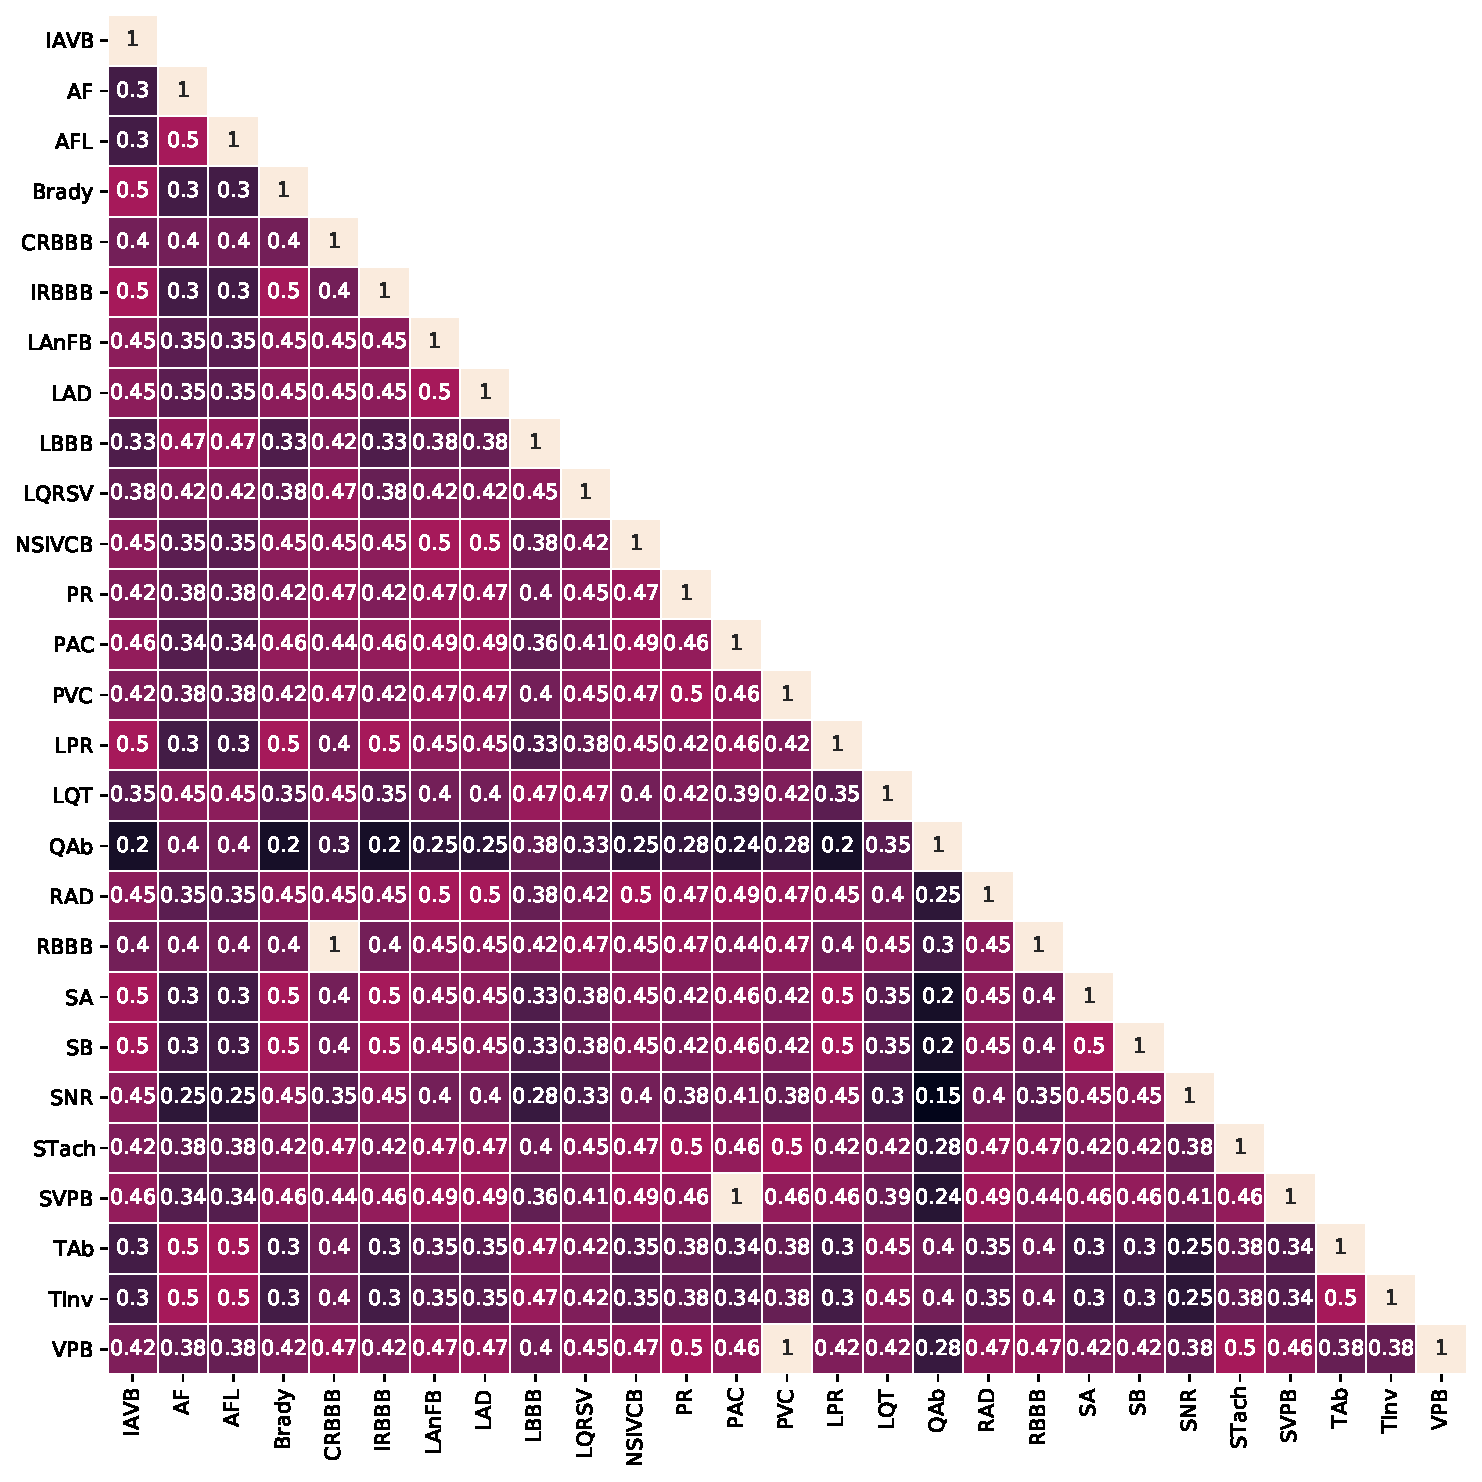
\includegraphics[trim={0.3cm 0.3cm 0.3cm 0.3cm},clip,width=8cm]{figure/aenc_label_weights.pdf}
    \caption{Evaluation scoring function weights per label.}
    \label{fig:dataset_labeldx}
\end{figure}

\begin{figure*}[tp]
    \begin{subfigure}[b]{0.66\textwidth}
        \centering
        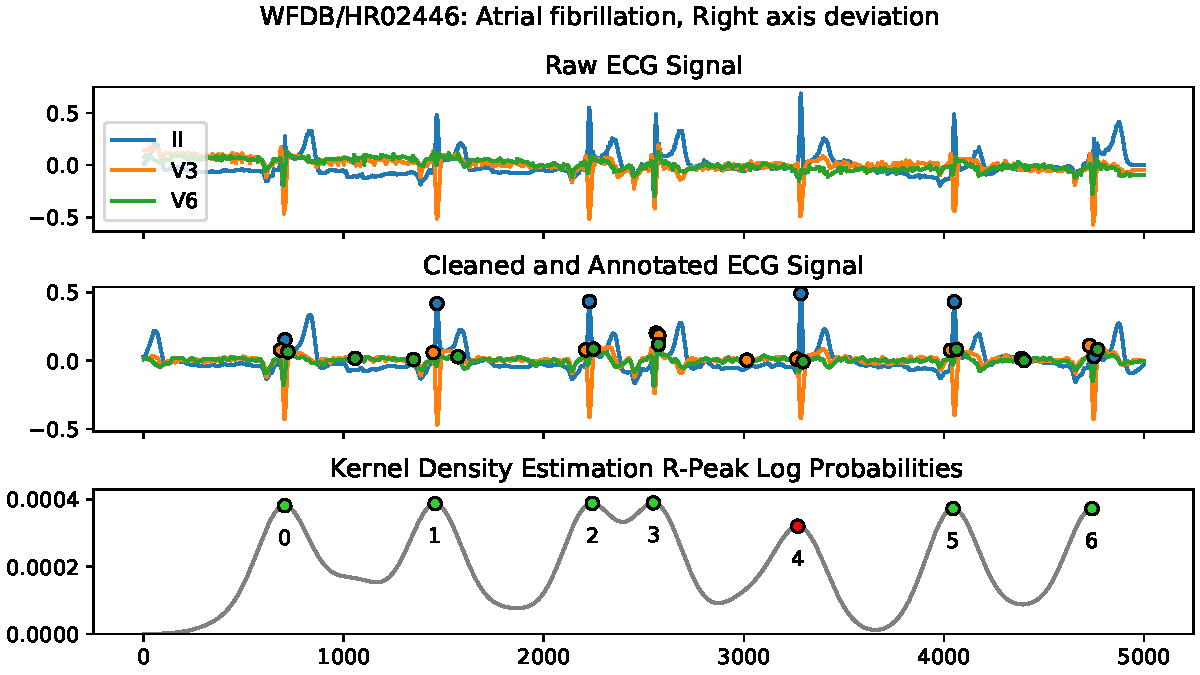
\includegraphics[width=\textwidth]{figure/aenc_3_sig_raw_clean_peaks.pdf}
    \end{subfigure}
    \begin{subfigure}[b]{0.33\textwidth}
        \centering
        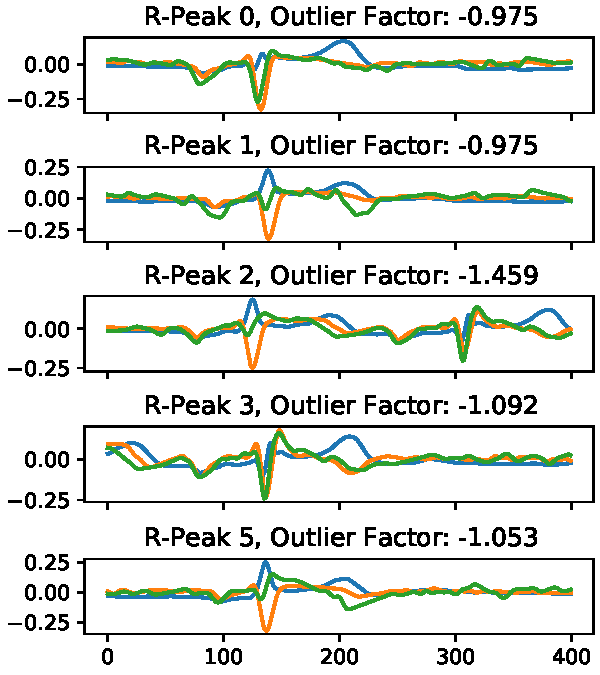
\includegraphics[width=\textwidth]{figure/aenc_3_sig_r_peak_windows.pdf}
    \end{subfigure}
    \caption{Signal processing from the raw signal to the annotated intermediary signal, to output heartbeat windows. Window 4 is dropped due to the cutoff threshold. Window 6 is dropped due to insufficient window size. Window 2 is the most abnormal heartbeat with the minimum outlier factor of the given windows. Only 3 of the 12 leads (\texttt{II}, \texttt{V3}, and \texttt{V6}) are shown for clarity.}
    \label{fig:signal_preprocessing}
\end{figure*}

\subsection{Signal Preprocessing}

We use the \emph{NeuroKit2} (v\texttt{0.0.40}) neurophysiological signal processing library~\cite{neurokit2} to annotate our ECG signals and the \emph{SciPy} (v\texttt{1.5.2}) family of Python packages for signal filtering and statistical tests~\cite{2020SciPy-NMeth}.
The ECG cleaning approach removes slow drift and DC offset using a Butterworth highpass filter (5Hz, $Q=0.5$) then smooths the signal using a moving average kernel of 0.02 seconds.
The R-peaks, or heartbeat locations, are annotated for each of our 12 signals.

Due to variable quality of sensor placements or noise artifacts caused by patient movements, the independent heartbeat annotations per channel may not be congruent within the ECG record.
We address this limitation with a kernel density estimation function fitted to the indices of all the R-peak annotations.
The bandwidth is the mean channel-wise heart rate multiplied by a $\frac{1}{4}$ scaling factor.
Next, we determine the peaks in the R-peak probability densities by finding all local maxima relative to their neighboring values.
We apply a cutoff threshold, dropping peaks that are over two standard deviations away from the mean peak value.

Given the overall R-peak indices for our 12-channel signal, we resample the entire signal such that the mean distance between each R-peak is 400 samples.
We slice windows of size 400, positioning the R-peak to occur at one-third of the length, and ignoring windows that do not contain 400 samples.
An $l_2$ normalization step is applied on all remaining windows.
We use the Breunig \emph{et al.} local outlier factor algorithm~\cite{10.1145/335191.335388} to find the most abnormal heartbeat in the ECG.

Our signal processing steps allow us to extract $\mathcal{M}$ normalized, fixed size heart beat windows from arbitrary length 12-channel ECG records.
A full example of the entire signal processing and windowing procedure is provided in Figure~\ref{fig:signal_preprocessing}.

\subsection{Heartbeat Autoencoder}

We rely on the dimensionality reducing properties of autoencoders~\cite{hinton2006reducing} to encode our heartbeat windows into an embedding, then concatenate our embeddings to get a representation of the overall ECG.
Our heartbeat autoencoder converts our $12\times 400$ heartbeat windows into embeddings of size $768$.

\begin{table}[ht]
    \caption{\label{tab:heartbeat_autoencoder} Heartbeat autoencoder neural network architecture.}
    \vspace{2 mm}
    \centerline{\begin{tabular}{llr} \hline
    \textbf{Block} & \textbf{Modules} & \textbf{Output Shape} \\ \hline
    \multirow{3}{*}{Enc1} & Conv1d(12, 16, 164), & \multirow{3}{*}{[$\mathcal{M}$, 16, 237]} \\
        & BatchNorm1d(16),\\
        & ReLU(), Dropout(p=0.1) \\ \hline
    \multirow{3}{*}{Enc2} & Conv1d(16, 20, 128), & \multirow{3}{*}{[$\mathcal{M}$, 20, 110]} \\
        & BatchNorm1d(20), \\
        & ReLU(), Dropout(p=0.1) \\ \hline
    \multirow{3}{*}{Enc3} & Conv1d(20, 24, 64), & \multirow{3}{*}{[$\mathcal{M}$, 24, 47]} \\
        & BatchNorm1d(24), \\
        & ReLU(), Dropout(p=0.1) \\ \hline
    Enc4 & Flatten(), Linear(1128, 768) & [$\mathcal{M}$, 768]\\ \hline \hline
    \multirow{2}{*}{Dec1} & Linear(768, 1024), & \multirow{2}{*}{[$\mathcal{M}$, 1024]} \\
        & ReLU(), Dropout(p=0.1) \\ \hline
    \multirow{2}{*}{Dec2} & Linear(1024, 4800), & \multirow{2}{*}{[$\mathcal{M}$, 400, 12]} \\
        & View(400, 12), Tanh() \\ \hline
    \end{tabular}
    }
\end{table}

The encoder has 970,420 trainable parameters among three convolutional blocks followed by a linear layer to generate the embedding.
Each block contains a convolutional layer followed by batch normalization, a ReLU activation, and a dropout normalization layer.
The decoder architecture, with 5,707,456 trainable parameters, contains two linear layers separated by a ReLU activation and a dropout normalization layer with a Tanh nonlinearity applied to the outputs.
See Table~\ref{tab:heartbeat_autoencoder} for the heartbeat autoencoder architecture.

We use stochastic gradient descent (SGD) with 0.9 momentum, to optimize our mean square error (MSE) objective.
We cyclically oscillate our learning rate between $1.0 \times 10^{-3}$ and $1.0 \times 10^{-5}$.
Training stops if the validation loss fails to attain a new minimum value after 3 epochs or after 100 epochs.

\subsection{Embedding Sequence Autoencoder and Classifier}

\begin{figure*}[b]
    \centering
    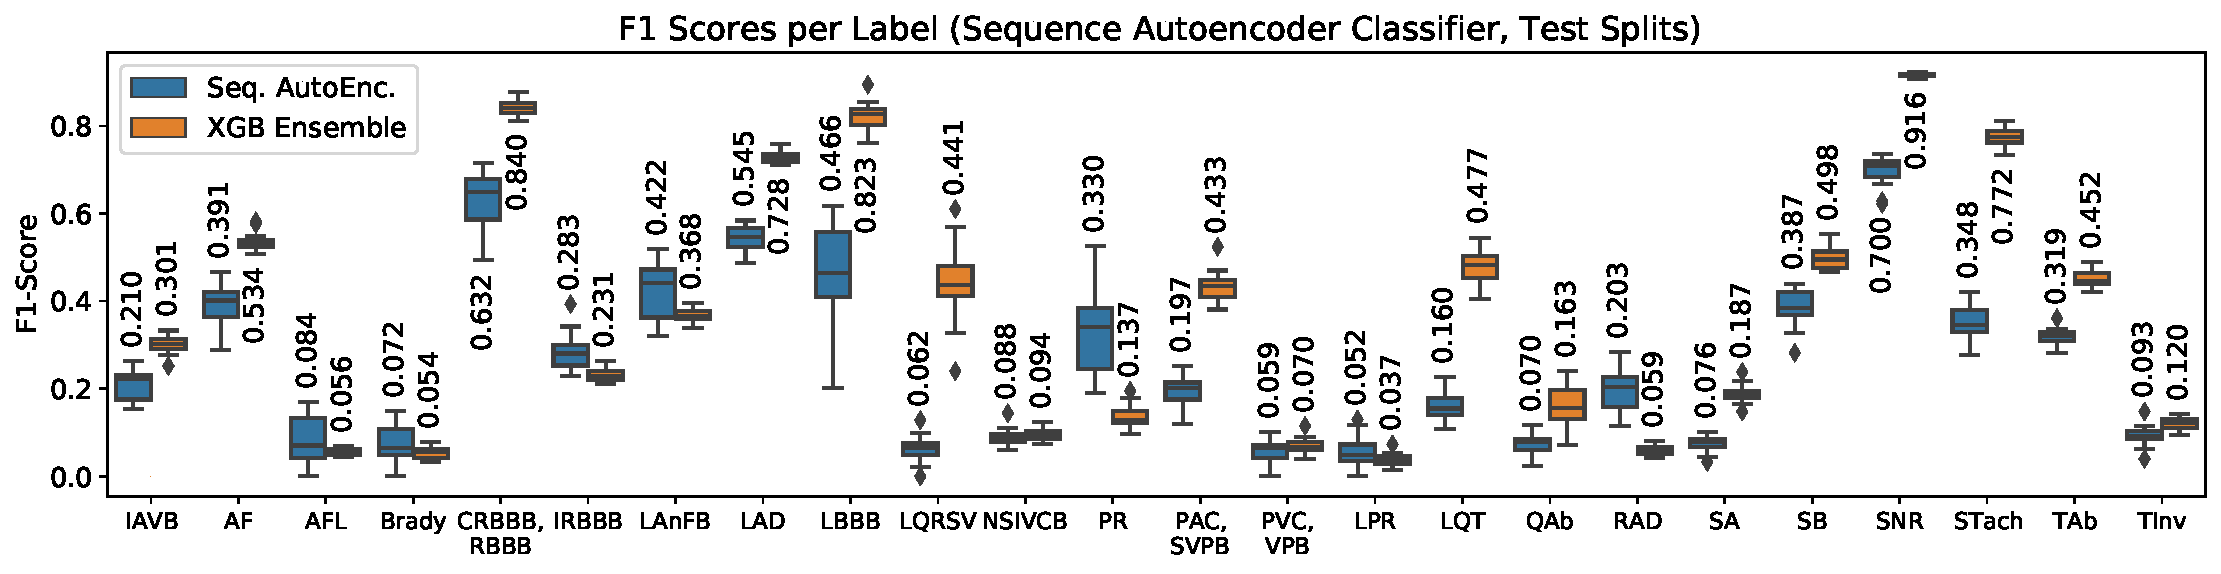
\includegraphics[trim={0.15cm 0.35cm 0.2cm 0.25cm},clip,width=\textwidth]{figure/aenc_label_f1s.pdf}
    \caption{Test set $\text{F}_1$ scores of all 27 labels compared with our prior XGBoost ensemble method~\cite{wong2020CINC-multilabel-ECG}. Mean values annotated.}
    \label{fig:label_f1s}
\end{figure*}

\begin{figure}[b]
    \centering
    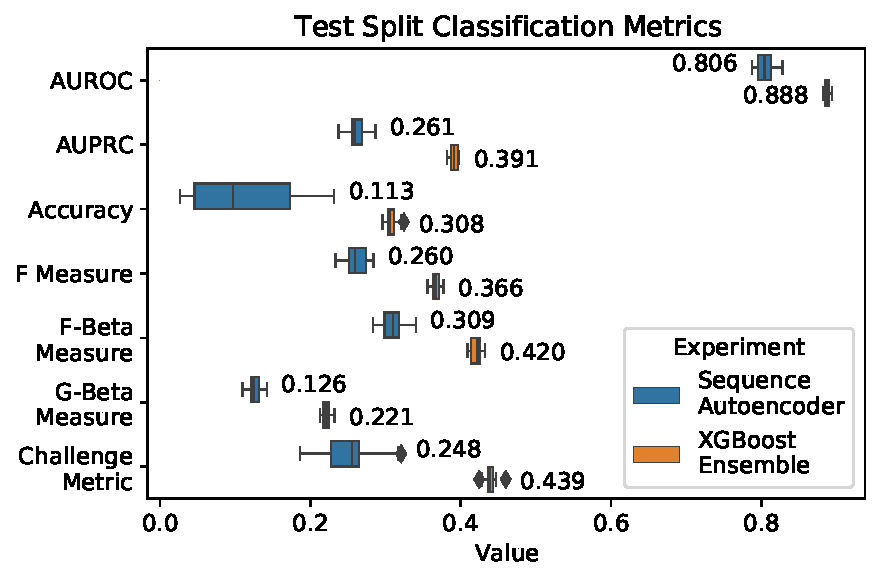
\includegraphics[trim={0.2cm 0.3cm 0.2cm 0.1cm},clip,width=8cm]{figure/aenc_classification_metrics.pdf}
    \caption{Classification metric summary of 20 experiments compared to XGBoost ensembles~\cite{wong2020CINC-multilabel-ECG}. Mean values annotated.}
    \label{fig:classification_metrics}
\end{figure}

The number of heartbeats extracted from an ECG record varies between 2 beats up to over 3,000 beats.
We limit this sequence length, capping the number of heartbeat embeddings used $\mathcal{M'}$ to 20.
Beginning with the abnormal heartbeat, we iteratively pick the rest of the candidate heartbeats by prepending the left neighbors and appending the right neighbors.
We stop when the neighbors are exhausted or 20 heartbeats are chosen.
For records with fewer than 20 beats, empty positions are masked and do not contribute to the loss.

% (lstm_enc): LSTM(768, 768, num_layers=2, dropout=0.1)
%   (lstm_dec): LSTM(768, 768, num_layers=2, dropout=0.1)
%   (seq_classifier): Sequential(
%     (0): Linear(in_features=768, out_features=256, bias=True)
%     (1): ReLU(inplace=True)
%     (2): Dropout(p=0.1, inplace=False)
%     (3): Linear(in_features=256, out_features=27, bias=True)
%   )
\begin{table}[ht]
    \caption{\label{tab:sequence_autoencoder} Sequence autoencoder and classifier architecture.}
    \vspace{2 mm}
    \centerline{\begin{tabular}{ll@{}r} \hline
    \textbf{Block} & \textbf{Modules} & \textbf{Output Shape} \\ \hline
    \multirow{2}{*}{Encoder} & LSTM(768, 768, & Hidden\\
        & num\_layers=2, dropout=0.1) & [768]\\ \hline
    \multirow{2}{*}{Decoder} & LSTM(768, 768, & Sequence \\
        & num\_layers=2, dropout=0.1) & [$\mathcal{M'}$, 768]\\ \hline
    \multirow{2}{*}{Classifier} & Linear(768, 256), ReLU() & Predictions \\
        & Dropout(p=0.1), Linear(256, 27) & [27] \\ \hline
    \end{tabular}
    }
\end{table}

The sequence autoencoder is symmetrical, with identical encoder and decoder architectures.
A two layer LSTM module with input and hidden sizes set to $768$ and dropout of $0.1$ is used, containing 9,449,472 parameters.
It encodes our $\mathcal{M'} \times 768$ heartbeat embeddings into a bottleneck of size $768$.
A multilayer perceptron consisting of two linear layers, separated by a ReLU and dropout layer ($p=0.1$) takes the sequence embedding of $768$, computes a hidden representation of $256$, and outputs $27$ label probabilities.
Our classifier has 203,803 parameters.
See Table~\ref{tab:sequence_autoencoder} for architecture design.

To mitigate internal validity risk the training, validation, and test splits are reused from the heartbeat autoencoder experiment.
Our pre-trained heartbeat encoder is frozen and does not update during the training of the sequence autoencoder.
We train the sequence autoencoder and classifier simultaneously using SGD and a cyclic learning rate.
Our overall loss function is the autoencoder MSE loss added to the binary cross entropy (BCE) classifier loss.
We scale the BCE weights to the count of negative samples over the positive samples in the training set split.

Training stops if the validation set challenge score fails to improve after 30 epochs or 200 epochs pass.
We use the highest validation set scoring model from all epochs and calculate the challenge metrics on the test set split, setting thresholds to maximize the training data receiver operating characteristic.

\section{Results and Discussion}

% All sequence autoencoders early stopped, running a mean of $70.75$ (std. $22.6$) epochs.
We compare our results with our prior XGBoost ensemble classifier~\cite{wong2020CINC-multilabel-ECG}.
Label-wise test $F_1$ scores can be found in Figure~\ref{fig:label_f1s}.
% Our methodology attains the highest $F_1$ mean values for normal sinus rhythm (SNR, $\bar{\text{F}}_1=0.700$), complete right bundle branch block (CRBBB \& RBBB, $\bar{\text{F}}_1=0.632$), and left axis deviation (LAD, $\bar{\text{F}}_1=0.545$).
Using the Wilcoxon signed rank test, our autoencoder $F_1$ means statistically outperform our prior work in detecting incomplete right bundle branch block (IRBBB, $p=1.9\times10^{-6}$), left anterior fascicular block (LAnFB, $p=9.4\times10^{-3}$), pacing rhythm (PR, $p=1.9\times10^{-6}$), and right axis deviation (RAD, $p=1.9\times10^{-6}$).
% Our autoencoder can effectively detect disorders dependant on heartbeat shapes, but additional work is required to represent the overall signal.

Overall test classification metrics is shown in Figure~\ref{fig:classification_metrics}.
Our methodology achieves a test split mean \emph{PhysioNet/CinC 2020 Challenge} score of $0.248$, AUROC of $0.806$, AUPRC of $0.261$, accuracy of $0.113$, macro $\text{F}_1$ score of $0.260$, $\text{F}_\beta$ of $0.309$, and $\text{G}_\beta$ of $0.126$ using $\beta = 2$.
Our autoencoder is worse than our shallow classifier on all summary metrics.
Our results cannot be compared with official rankings because the challenge evaluates the algorithms on secret hold-out test sets.
% Our label-wise $\bar{\text{F}}_1$ is correlated with the label frequency (Pearson $r=0.655$, $p=5.1\times10^{-4}$) despite the scaling of the dataset label weights.
% The collection and synthesis of new ECG records of low occurrence disorders to use as training data may improve future classifiers.

Our methodology trains a neural network using the general shapes of heartbeat windows and indirectly models the overall signal by looking at consecutive heartbeats.
Consequentially, due to the variable distances of the R-peaks within an ECG record, portions of the ECG signal not bounded between a heartbeat window are dropped.
Because we resample the overall signal to ensure heartbeat windows are 400 samples long, we drop heart rate information.
Currently we do not capture features like average heart rate or changes in heart rate over time.
Additionally, because of the $l_2$ normalization of the heartbeat windows, we also do not capture the original signal amplitudes and voltage changes.
Future work should expand on our findings to incorporate heart rate velocities, raw amplitudes, and continuous full signal characteristics.
% Our classifiers continue to require human oversight before use in the healthcare setting~\cite{10.1145/3233547.3233667}.

\section{Conclusion}

Using a signal processing and heartbeat window extraction preprocessing step, we train heartbeat autoencoders to be fed into ECG sequence autoencoders before training a multi-label perceptron to classify 27 heart conditions.
We run $20$ independent experiments, randomly sampling our available dataset into 80\% training, 10\% validation, and 10\% test set splits.
Our methodology achieves a mean unofficial test challenge score of 0.248 with an overall macro $\text{F}_1$ score of 0.260.
    

\end{document}
